\documentclass{thesis}
%\usepackage{lgrind}
\usepackage{graphicx}
\usepackage{caption}
\usepackage{subcaption}
\usepackage{verbatim}

\usepackage[font=small,labelfont=bf]{caption}

\pagestyle{plain}
\bibliographystyle{apalike}
\renewcommand{\bibname}{References}

\begin{document}

\pagestyle{plain}
\title{Detecting Photo Manipulation using Reflections on Curved Surfaces}
\author{Laura A. Moss}
\date{}
\maketitle

\newpage

\subsection*{Abstract}
Abstract goes here
  % -*- Mode:TeX -*-
%% This file simply contains the commands that actually generate the table of
%% contents and lists of figures and tables.  You can omit any or all of
%% these files by simply taking out the appropriate command.  For more
%% information on these files, see appendix C.3.3 of the LaTeX manual. 
\tableofcontents
%\newpage
%\listoffigures
%\newpage
%\listoftables


% Body
\chapter{Introduction}

% TODO cases of forged images in journalism and science?

% TODO how long has the field been around?

% TODO examples of research


Image forensics, the study of finding hidden information in photographs, is an emerging field with diverse applications. It is comprised of a few general subtopics: determining the source of an image, detecting forgery, and detecting steganography (hiding information in a digital image) \cite{rocha2011}. All too often, pictures are used as hard evidence in journalism, scientific research, and criminal cases. For example, there was one incident in the scientific community in which a group of South Korean scientists published groundbreaking stem cell research results, but it was later revealed that the majority of the photographs included with the results were doctored \cite{rocha2011}. Image forgery itself predates the digital age, but as computers have become more capable and tools such as Adobe Photoshop have been developed, it has become much easier to manipulate images in a convincing manner. Therefore, there is an increasing need for forensic techniques as the technology develops.

Existing forensic techniques generally involve machine learning, finding statistical anomalies, or finding geometric inconsistencies. The current techniques that take advantage of reflective objects in an image fall into the latter category. Interestingly, the human eye is very insensitive to inconsistencies in reflections \cite{farid2010image}. Therefore it would be fairly straightforward for a forger to, for example, convincingly show a person in a scene with a reflective surface who was never actually there. It would perhaps be convincing to a human, but may not hold up to analysis with a geometric technique.

Most of the reflective surfaces that might be found in real photos are planar. Some common examples are bodies of still water, mirrors, and glass windows. Non-planar reflective surfaces, which are the focus of this paper, are less common but can be found in the form of store security mirrors, works of art, and even the human eye.

\chapter{Prior Work}
% intro
Prior research into geometric consistency in digital images has dealt most notably with shadows and planar reflective surfaces.
\section{Similar Geometric Techniques}
There are forensic techniques similar to reflection consistency that take a geometric approach to shadow consistency. Instead of determining if there is a consistent vanishing point, or a plausible consistent camera location (see Section~\ref{sec:planar-reflections}), these techniques determine if there is a consistent location for a light source. One simple technique for determining shadow consistency, akin to the techniques for reflection consistency, involve drawing rays between points on an object and corresponding points on the shadow. These rays should intersect in a plausible location for the light source (or they should be nearly parallel if the light source is the sun) \cite{farid2010image}. This is dependent on the shadows having easily distinguishable features that can be matched up to the object that is casting the shadow.

\begin{figure}[h]
	\centering
    	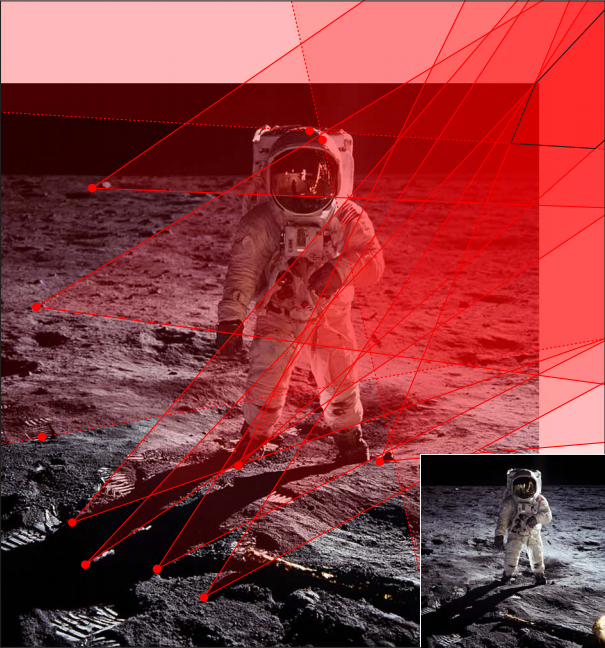
\includegraphics[width=0.8\textwidth]{moon-landing-consistent}
	\caption{Based on shadow wedge constraints, this photo of the moon landing has a consistent light source. Original image copyright 1969, NASA. \cite[Fig.~1]{kee2013exposing}}
	\label{moon-landing-consistent}
\end{figure}

Another similar technique improves on the previous one by eliminating the need for distinguishable shadow features. Instead of drawing rays, a point is picked on a shadow and a wedge constraint created that contains all of the object that could have plausibly cast that point of the shadow \cite{kee2013exposing}. If there exists a region that satisfies all the constraints, the image passes this test, as in Figure~\ref{moon-landing-consistent}.

\section{Reflections on Planar Surfaces}
\label{sec:planar-reflections}
\begin{figure}[h]
	\centering
    	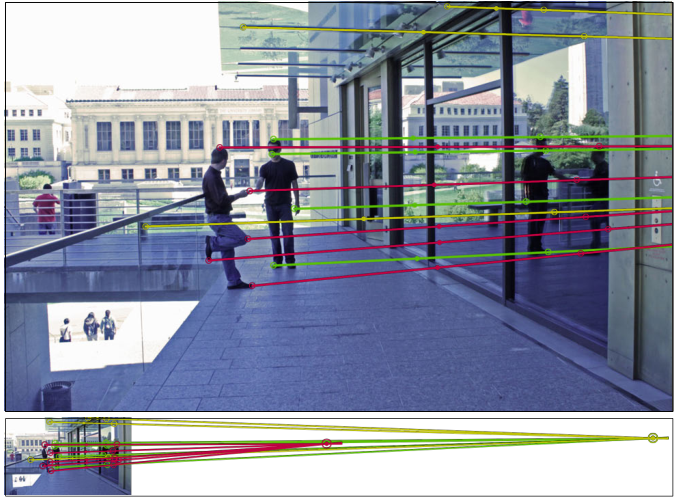
\includegraphics[width=0.8\textwidth]{planar-vanishing-point-forged}
	\caption{Demonstration of vanishing point inconsistency. The lines corresponding to the man on the left converge to a different vanishing point than those from the rest of the scene, so it is likely that the man and his reflection were edited into the scene. \cite[Fig.~1]{obrien12}}
	\label{planar-vanishing-point-forged}
\end{figure}

\begin{figure}[h]
	\centering
    	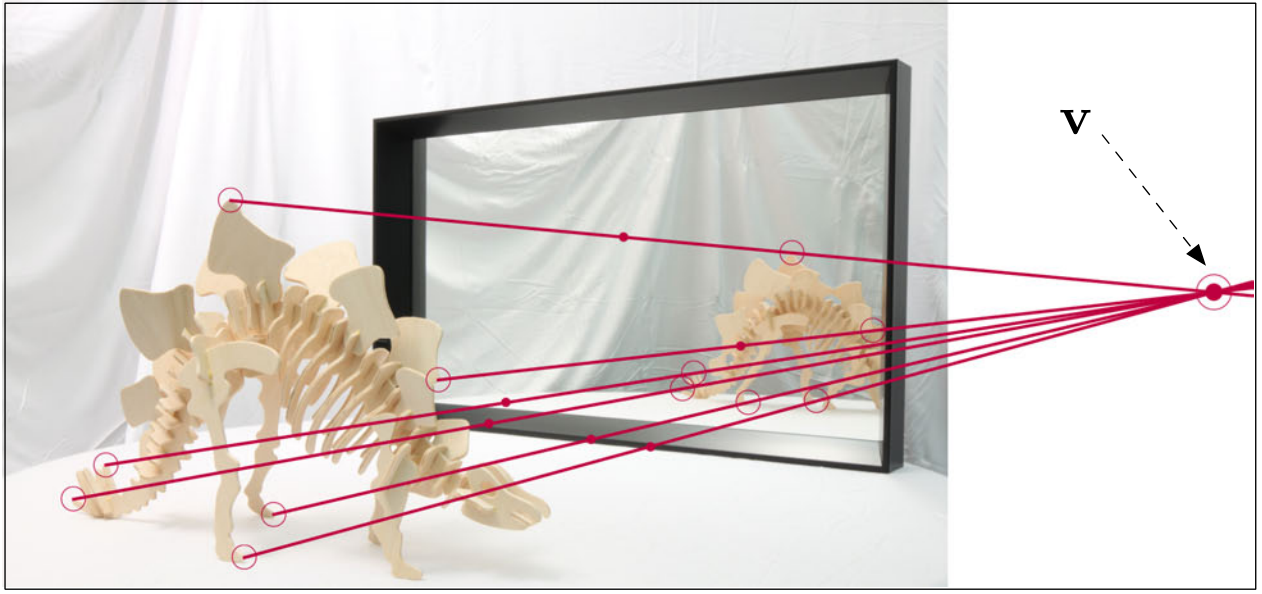
\includegraphics[width=0.8\textwidth]{planar-midpoint-genuine}
	\caption{Demonstration of midpoint and vanishing point consistency. The lines converge to a well-defined vanishing point $V$. Additionally, the midpoints in three-dimensional scene space between the real and reflected features plausibly intersect the mirror plane. \cite[Fig.~3]{obrien12}}
	\label{planar-midpoint-genuine}
\end{figure}

\begin{figure}[h]
	\centering
    	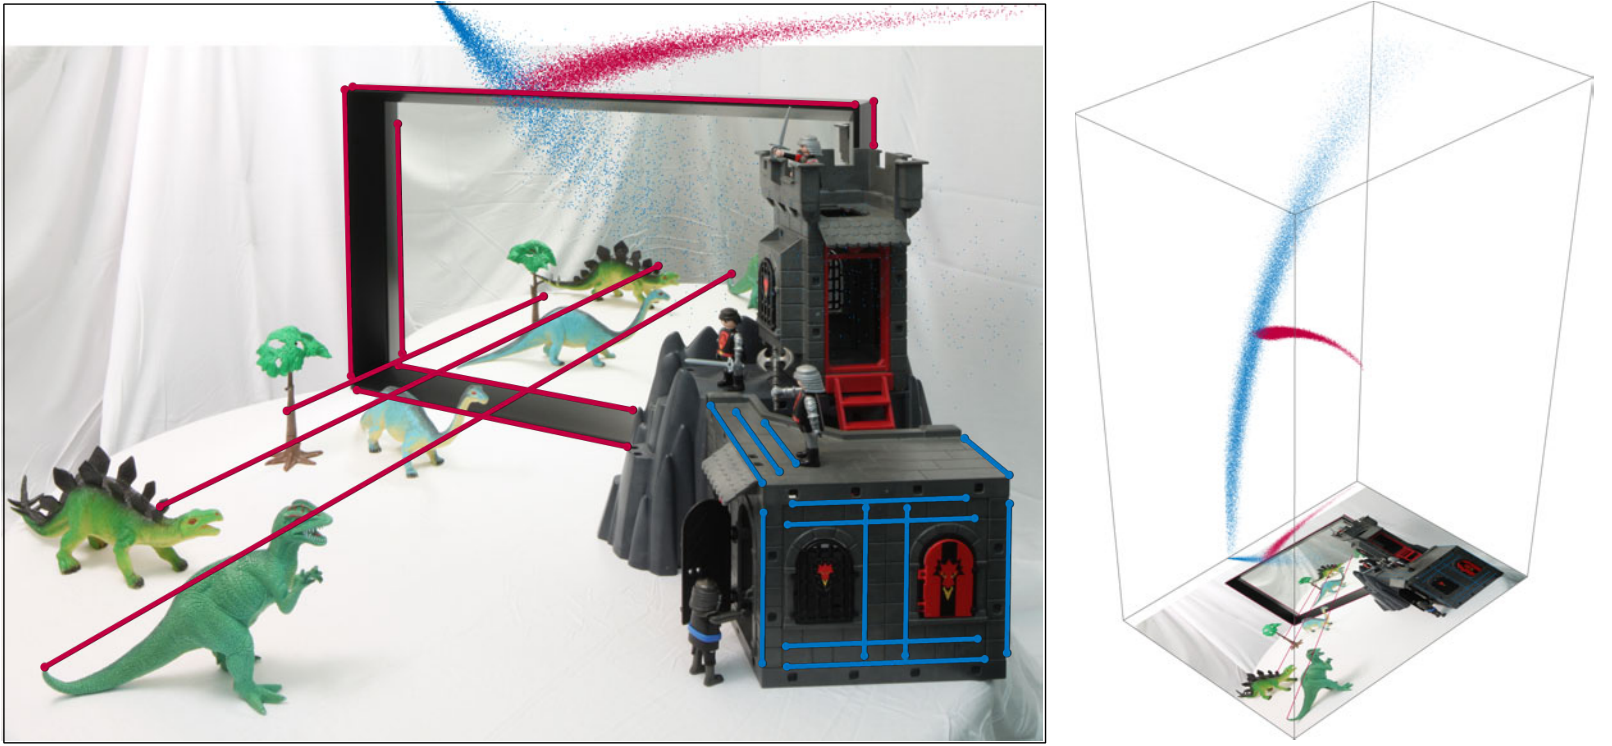
\includegraphics[width=0.8\textwidth]{center-of-projection-planar-genuine}
	\caption{Demonstration of center of projection consistency. The pink and blue point clouds represent sets of possible solutions, generated by randomly perturbing the points selected that form the lines. Since the point clouds intersect, there is a possible consistent center of projection, or camera position. \cite[Fig.~6]{obrien12}}
	\label{center-of-projection-planar-genuine}
\end{figure}

Recent research into properties of images that can be exploited to find inconsistencies has shown that an object in an image and its reflection in a mirror must have certain geometric properties in a real, unmanipulated image. O'Brien and Farid's 2012 paper discusses several techniques for determining whether or not an image that contains a planar mirror is consistent.\nocite{obrien12} All of these techniques are derived directly from linear perspective projection geometry.

The first step to all of the techniques is obtaining lines in the image that are parallel in three-dimensional scene space (or should be if the image is genuine). The first couple of techniques require hand-picking matching points between the original objects in the scene and their virtual (reflected) counterparts. Then, straight lines are drawn connecting these point pairs out to infinity. These lines, if drawn through the same planar mirror, must all intersect at a single vanishing point. If they don't intersect cleanly, or intersect at multiple vanishing points, the image can be assumed to be forged, as seen in Figure~\ref{planar-vanishing-point-forged}. Furthermore, the midpoints of the same lines in three-dimensional scene space must also plausibly appear to intersect the reflective surface, as in Figure~\ref{planar-midpoint-genuine}. Finally, as in Figure~\ref{center-of-projection-planar-genuine}, if there are orthogonal parallel lines in the image (for example, on the frame of a mirror), we can check if there is a consistent position for the center of projection, or point camera.

If a forger wanted to manipulate an image that contains a reflective surface, they would likely be trying to create a composite of images. For example, if they were trying to place a person in the scene that was never actually there, they would paste in that person and their reflection from another image. It may be relatively simple to align and resize these components so that they look convincing in the new image, but the reflection may still retain some properties of the mirror in the image it came from.



% TODO section describing approach? including assumptions and why they are reasonable, overview of tools

\chapter{Mathematical Techniques}
\section{Approach}
The goal of this analysis is to find a method for determining reflection consistency that is general enough to not require knowledge of the camera parameters, in the same vein as the existing techniques for planar mirrors. To simplify the geometry of this analysis, we will restrict the form of our non-planar mirrors to be spherical. Quadric surfaces in general are likely to be good enough for typical use cases because most general curves encountered in the real world can be approximated as either a quadric surface or a set of quadric surfaces.

We also assume the camera used to take any of the images analyzed is a point camera with perspective projection. This is a reasonable assumption considering both the size of most digital camera sensors, and the fact that the camera would have to be far enough away from the subjects of the photograph to capture everything required to perform the analysis.

An important idea to note is that showing that an image is consistent according to these techniques is not sufficient to prove that the image is genuine, because the image could have had some counter-forensic techniques applied or been manipulated in a way that is unrelated to reflective geometry.

\section{Properties of Reflective Geometry}
% expanded to sync up nomenclature
Reflection of light on a surface is directly related to the surface normal at the point of reflection. The incident ray (or ray of light coming towards the surface) must make the same angle with the normal as the reflected ray.  Additionally, the incident ray, reflected ray, and normal must all be coplanar, and the reflected and incident rays must be on opposite sides of the normal. In 3D space, we can call the point being reflected $P$ and the reflection point $R$. Then the incident ray in 3D space is $PR$, and the projection of $P$, $R$ and $PR$ onto the image plane are $p$, $r$, and $pr$. $pr$ will be referred to as the projection of the incident ray.

\begin{figure}
	\centering
    	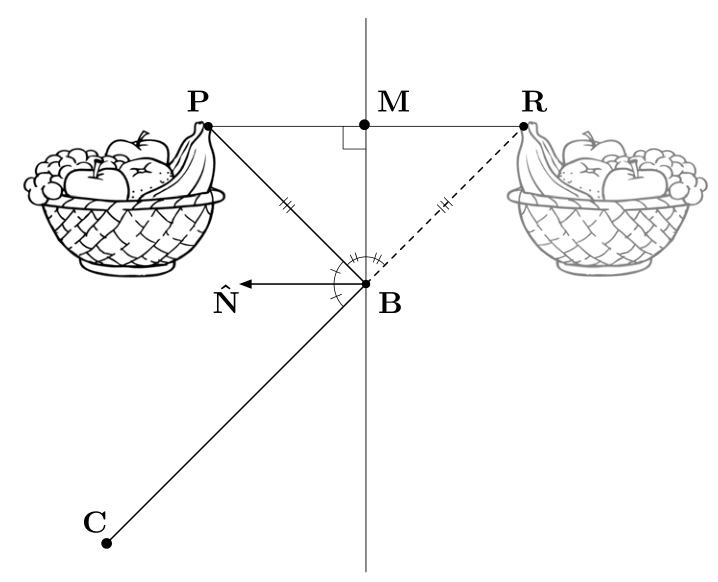
\includegraphics[width=0.6\textwidth]{normal-reflection}
	\caption{Given a camera location $C$, a point $P$ on an object and its corresponding reflection $R$, the ray $PR$ appears equivalent to the ray $PB$ from the point of view of the camera. The ray $PR$ is also parallel to the surface normal $\hat{N}$. Since all of the points in this diagram must be coplanar, this holds true in 3D space. \cite[Fig.~2]{obrien12}}
	\label{normal-reflection}
\end{figure}

O'Brien and Farid point out that a non-obvious consequence of this law is that if a ray is drawn between the reflected object and its reflection, it should appear to be parallel to the surface normal at the point of reflection. (In the planar case, it would appear perpendicular to the mirror, since the normal is constant over the whole surface.) We will call this the projection of the incident ray. Furthermore, the incident ray and the ray drawn between the reflected object and its reflection's apparent location are co-linear from the perspective of a point camera, as demonstrated in Figure~\ref{normal-reflection}. This is why drawing rays on a picture between an object and its reflection works: it appears equivalent to drawing rays to the apparent position of the reflected object.

In the case of a planar mirror, all of these rays would be parallel in three-dimensional space.\nocite{obrien12} An axiom of linear perspective projection is that parallel lines projected onto a 2D image must converge to some vanishing point $V$ \cite[p.~2]{hartley}, so all such lines through a planar mirror intersect at a single vanishing point if the photograph is unaltered. This is the mathematical basis for the technique described in Section~\ref{sec:planar-reflections}.


\section{Reflective Sphere Geometry}
\begin{figure}
	\centering
    	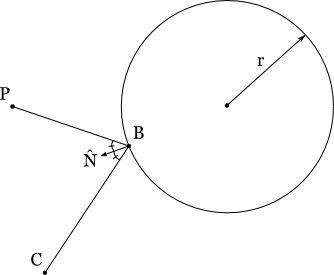
\includegraphics[width=0.6\textwidth]{colinear-radius}
	\caption{Since the point $P$, the reflection point $B$, the camera $C$, and the normal $\hat{N}$ are all coplanar, and $\hat{N}$ is an extension of the radius of a sphere, then $PB$ and any radius on this cross-section of the sphere must be coplanar.}
	\label{colinear-radius}
\end{figure}

\begin{figure}
	\centering
    	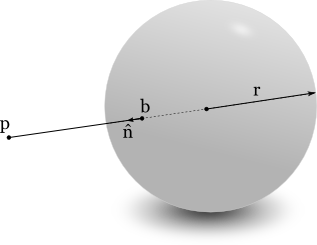
\includegraphics[width=0.6\textwidth]{colinear-radius-camera-view}
	\caption{A view of Figure~\ref{colinear-radius} from the viewpoint of the camera $C$.}
	\label{colinear-radius-camera-view}
\end{figure}

In the case of a curved surface, the ray to the apparent position of the reflection is still parallel to the normal at the point of reflection. Unlike a planar mirror, since the normal is not constant, all such rays through the same mirror will not be parallel in three-dimensional space.

If the curved surface happens to be spherical we can exploit the fact that the normal at any point on the surface is colinear with some radius of the sphere. This is because any normal on a sphere points directly away from the center of the sphere. Since the incident ray, reflected ray, and normal are all coplanar, and the normal and the radius are coplanar, then the incident ray and any radius in that cross-section of the sphere are coplanar [Figure~\ref{colinear-radius}].

From the view point of the camera, since the projection of the incident ray is colinear with the normal, it must also be colinear with the radius. Therefore, in theory, in a valid picture of a reflective sphere any incident ray must appear to pass through the center of the sphere [Figure~\ref{colinear-radius-camera-view}].

\section{Why not estimate the normal?}
\label{sec:normal-estimate}
In general, the types of techniques outlined verify that the incident ray is consistent with the normal at the point of reflection. If the projection of the normal could be estimated on any arbitrary image of a quadric surface, then we could easily have a technique to detect inconsistencies in reflections on most curved surfaces because the projection of the normal and the projection of the incident ray should be colinear. However, when perspective projection is taken into account, it is non-trivial to estimate the normal accurately on an arbitrary visible point on the surface, even for a simple surface like a sphere.

In the unrealistic case where an image was produced using orthographic projection, the projection of the normal could be easily estimated on a sphere because the sphere appears exactly the same no matter the angle from which it is viewed, and the entire hemisphere facing the camera is visible. The $x$ and $y$ components of the projection of the normal vector are simply a function of the projection of the position on the sphere. With perspective projection, the visible region of the sphere is slightly smaller than the projection of the hemisphere so the radius can not be determined from the visible size of the sphere alone.

% explain that camera parameters are needed
If the camera parameters were known (which is outside the scope of this paper), the normal could be estimated anywhere on the visible part of the sphere. Knowing the camera parameters implies that we know exactly where the center of projection is relative to the image plane. If we fit an ellipse to the apparent contour of the sphere (see Section \ref{sec:perspective-distortion} for details on why it is an ellipse), we get an elliptic cone formed by the center of projection and the ellipse \cite[p. 201]{hartley}. There is then a family of spheres that fit into the cone that could possibly have created the apparent contour (with increasing radius as the sphere gets farther away). Since the normals on any sphere in the family map to the image plane the same way, it is sufficient to know the cone to find the normals.

\section{Why not find the midpoints?}
In the case of a nonplanar mirror, we lack something that is easily obtainable in the planar case: a vanishing point for the incident rays. Thus, we can't find the midpoints in 3D space for the incident rays for a spherical mirror by the same method. It may be possible to find the midpoint by constraining the 3D incident ray to lie between the rays from the camera to the point and its reflection, then restricting the midpoint to both bisect the incident ray and the ray to be colinear with the normal. Again, however, this requires that the camera parameters be known.

\chapter{Implementation}
In order to expedite the process of obtaining images that meet a variety of very specific conditions, all images used to test these algorithms were computer-generated using Blender 2.68a.

The application consists of a Python script that uses PySide for GUI and drawing, and Numpy and Scipy for mathematical calculations. It has an interface for a user to locate a circle and its center, and to locate projections of incident rays.

\section{Circle Finding}
To find the center of the sphere, the user picks several points (at least 3, depending on the configuration of the program) along the visible edge of the sphere. The application then finds the best fit for the radius and center of a circle given the points picked.

Because accuracy in finding the sphere center is key to this analysis, the application employs some rudimentary edge detection to assist in picking points on the edge of the sphere. Based on an initial point picked, it examines several pixels towards and away from an initial guess for the center and moves the point halfway between the pixels with the greatest difference in color. This edge detection is fairly limited, but is good enough for the purpose of the test images used because of their plain and easily distinguishable colors.

\subsection{Distortion from Perspective Projection}
\label{sec:perspective-distortion}

\begin{figure}
	\centering
    	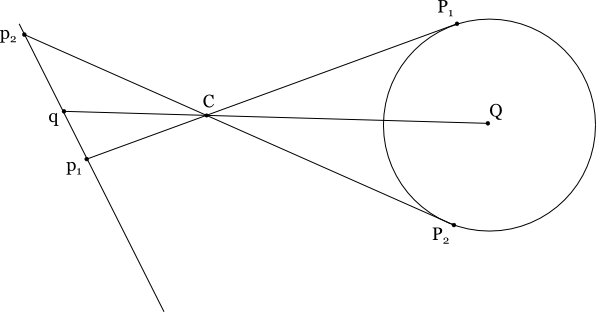
\includegraphics[width=0.6\textwidth]{sphere-distortion}
	\caption{If the image plane is not facing the sphere head-on, the distance from the point $P_2$ to its projection $p_2$ through the center of projection $C$ is shorter than the distance from $P_1$ to $p_1$, so $P_2$ appears closer and thus that side of the sphere appears larger. Additionally, the projection $q$ of the sphere center $Q$ is not the midpoint of $p_1$ and $p_2$.}
	\label{sphere-distortion}
\end{figure}

\begin{figure}
	\centering
	\begin{subfigure}[b]{0.4\textwidth}
                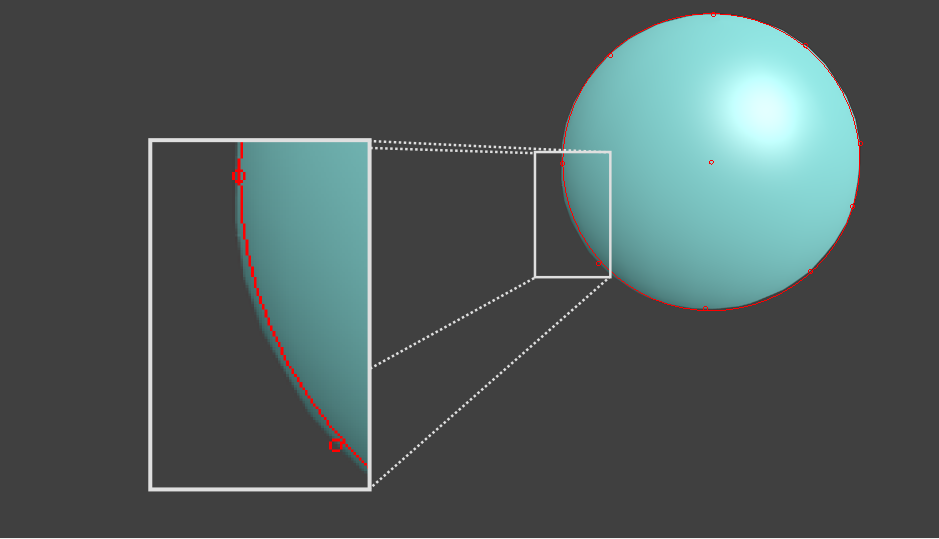
\includegraphics[width=\textwidth]{sphere-perspective-zoom}
                \caption{Perspective view of a sphere}
    \end{subfigure}
    ~
   	\begin{subfigure}[b]{0.4\textwidth}
                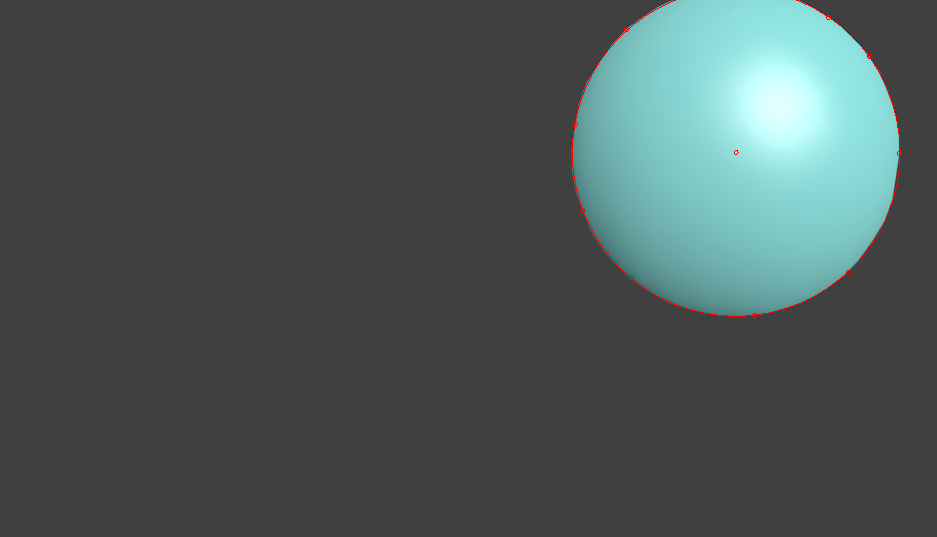
\includegraphics[width=\textwidth]{sphere-ortho}
                \caption{Orthographic view of a sphere}
    \end{subfigure}
    \caption{Viewing the sphere with perspective projection introduces noticeable error when solving for the circle projected onto the image plane.}
	\label{sphere-perspective-ortho}
\end{figure}

One issue with this naive approach to finding the center is that perspective projection distorts the shape of the sphere, depending on how centered the sphere is in the camera's view. If the sphere is towards the edge of the camera's view, the extent of the visible part of the sphere towards the edge is closer to the camera than the visible extent of the part of the sphere towards the middle of the image. This causes the sphere to look larger towards the edge of the image and therefore the apparent edge of the circle distorts out towards the edge of the image. This effect is described in Figure~\ref{sphere-distortion}. As a result, the outline projected onto the image is slightly elliptical, as in Figure~\ref{sphere-perspective-ortho}. If the camera parameters were known, we could just estimate the normal at any point as outlined in Section~\ref{sec:normal-estimate}.

% IRL example of this phenomenon?
% example with smaller sphere?



\chapter{Results}
\begin{figure}[h]
	\centering
    	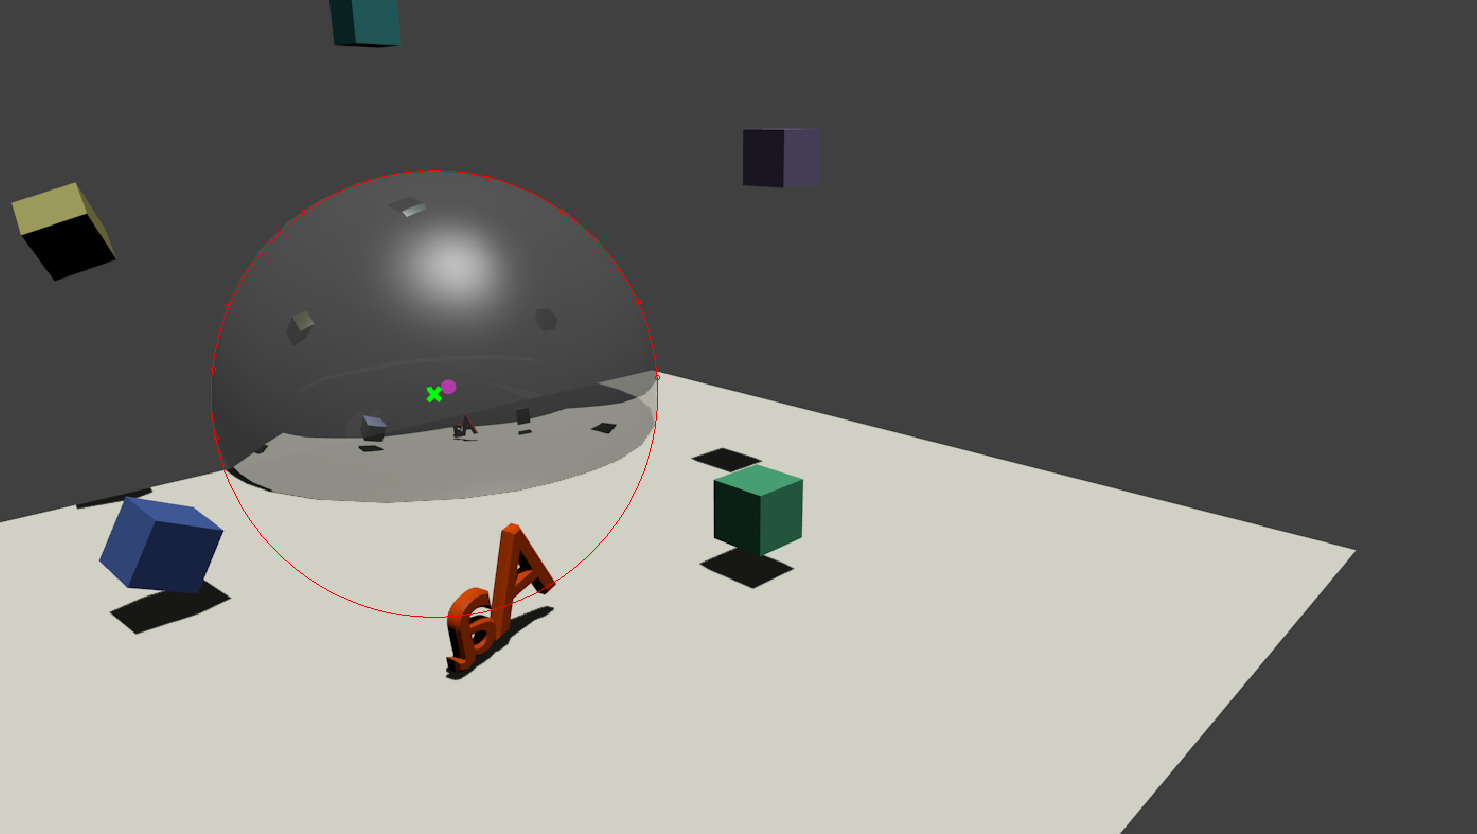
\includegraphics[width=0.8\textwidth]{center-error}
	\caption{The center found when finding the best fit for a perfect circle (green cross) is significantly offset from the actual projected center of the sphere (pink dot).}
	\label{center-error}
\end{figure}

As detailed in Section~\ref{sec:perspective-distortion}, it as not as simple as finding the outline of a perfect circle to find the projection of the center of the sphere in the image. Therefore, for the purpose of testing the method, test images were generated with a small sphere located at the exact center of the reflective sphere made slightly transparent. Figure~\ref{center-error} shows how inaccurate the naive center-finding method can be.

Because there is some error associated with having a human input the points to create the projections of the incident rays, it is assumed that in an unaltered image the rays will probably not cross the exact center of the sphere. For this reason, the measure for authenticity will be how close the rays come to the center of the sphere.

One possible alternative to looking at the minimum distance to the center would be to consider the the point of intersection of all the rays, similar to the vanishing point method in the planar case. However, the spherical case is much more sensitive to error than the planar case. In the planar case the incident rays are parallel, so their vanishing point often lies far outside the image, and so the position of the intersection point is not very sensitive to a difference of a few pixels in the points picked. In the spherical case, however, it is not uncommon for the projections of the incident rays to not intersect cleanly even in genuine images.

The primary test set includes Blender-generated images of a smaller sphere with surrounding objects that are close, moderately far away, and very far away, and likewise for a larger sphere.

% measurable error- residuals?

\section{Typical Results for Genuine Images}
\begin{figure}[h]
	\centering
    	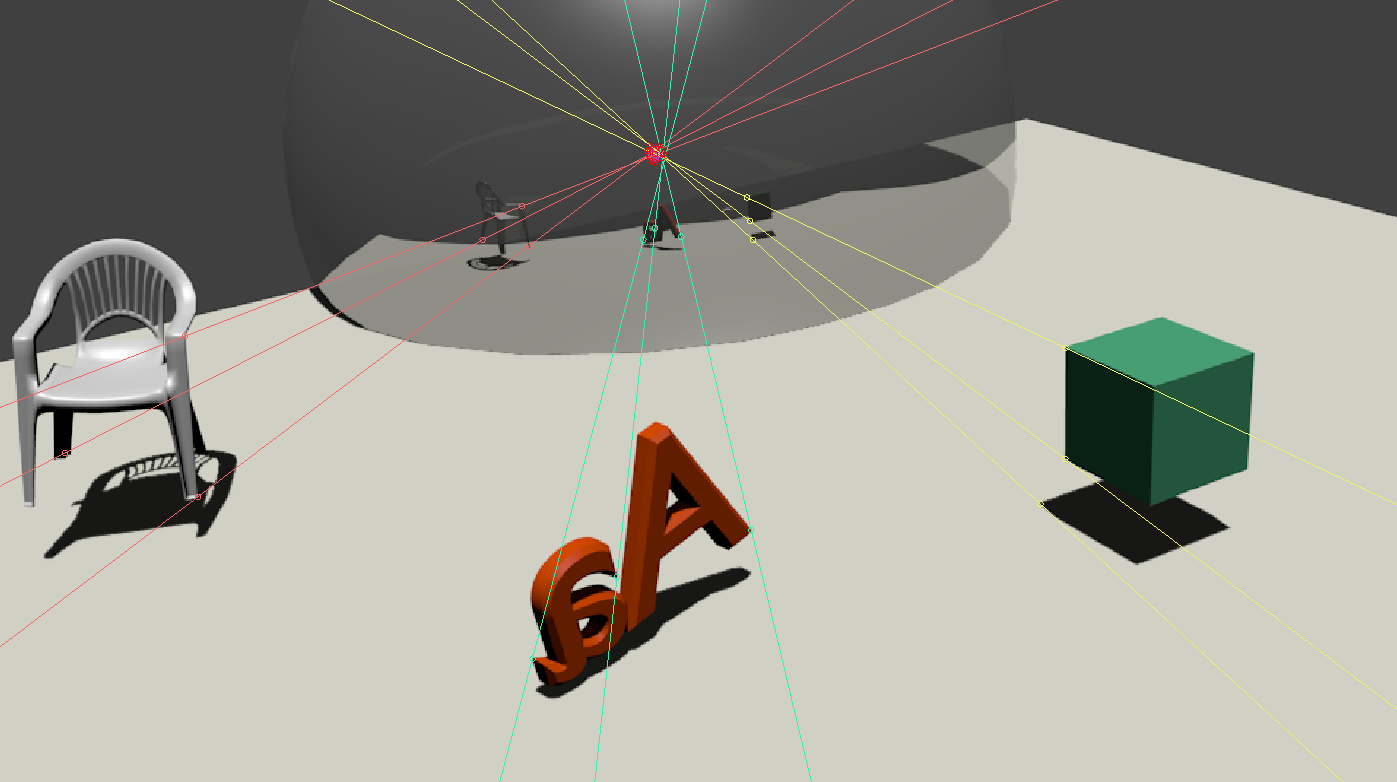
\includegraphics[width=0.6\textwidth]{1b-genuine}
	\caption{The chair and the cube are reasonably consistent with the center of the sphere, but the incident rays from the letters appear to intersect at a point slightly offset from the center, despite being unmanipulated.}
	\label{1b-genuine}
\end{figure}

\begin{figure}
	\centering
	\begin{subfigure}[b]{0.4\textwidth}
                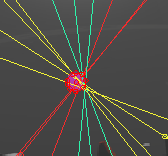
\includegraphics[width=\textwidth]{lo-res-detail}
                \caption{960x540, detail}
    \end{subfigure}
    ~
   	\begin{subfigure}[b]{0.4\textwidth}
                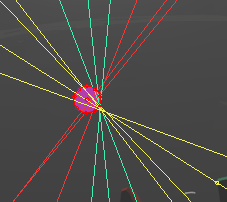
\includegraphics[width=\textwidth]{hi-res-detail}
                \caption{1920x1080, detail}
    \end{subfigure}
    \caption{Increasing the resolution does not significantly improve the distance from the incident rays to the center, which implies that there is some other phenomenon at work.}
	\label{resolution-comparison}
\end{figure}
Overall, in practice for the test set of images, the projections of the incident rays come fairly close to the sphere center, which would seem to support the validity for this consistency test. In most images, the rays all come within 10 pixels of the sphere center. However, the rays have a consistent offset from the center, which indicates that there may be some other phenomenon at work. For example, in Figure~\ref{1b-genuine}, some objects seem to have a clean intersection point that is offset from the sphere center. This location for the intersection is consistent for multiple trials of analyzing the image, so it is clearly not the result of random human error when picking points.

Some images appear to contain more error than others. In the test set, the images with the smaller reflective sphere have the rays clustered more tightly around the sphere center than those with the larger sphere. For an image of a small sphere with objects at medium distance, the rays were often within 2 pixels of the center, but away as much as 4 pixels, For the analogous image with the larger sphere at the same resolution the rays were mostly within 3 pixels but as far away as 7. The effect is slight but fairly consistent.

The resolution of the image also has an effect on the distance to the center from the rays. A test image was rendered in Blender at both an original resolution of 960x540 and 1920x1080, or double the original resolution (Figure~\ref{resolution-comparison}). The increase in resolution resulted in an overall increase in pixel distance, though the pixel distance did not double. The fact that the distance did not double indicates that having more detail does lead to more precision in selecting features, as expected. The fact that it did not decrease, however, indicates that there is some naturally occurring offset in the image that is not the result of human error.

One other consideration that was explored is whether or not point picking introduces some constant error. Flipping the image horizontally or vertically and then analyzing it also flips the direction of the offset, so this is clearly not the case.


\section{Effects of Forgery}

\begin{figure}
	\centering
    \begin{tabular}{c c}
	    \begin{subfigure}{0.45\textwidth}
	                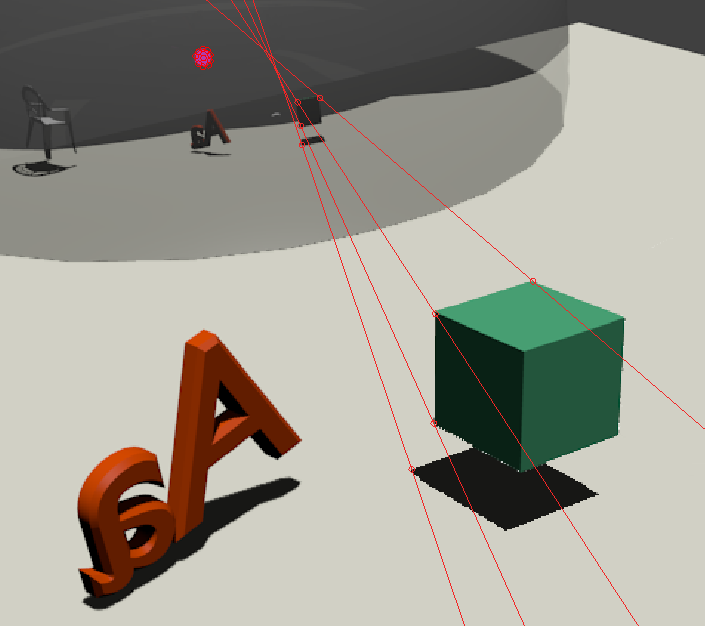
\includegraphics[width=\textwidth]{1b-lateral}
	                \caption{Movement about the sphere\\}
	                \label{subfig:1b-lateral}
	    \end{subfigure}
	    &
	    \begin{subfigure}{0.45\textwidth}
	                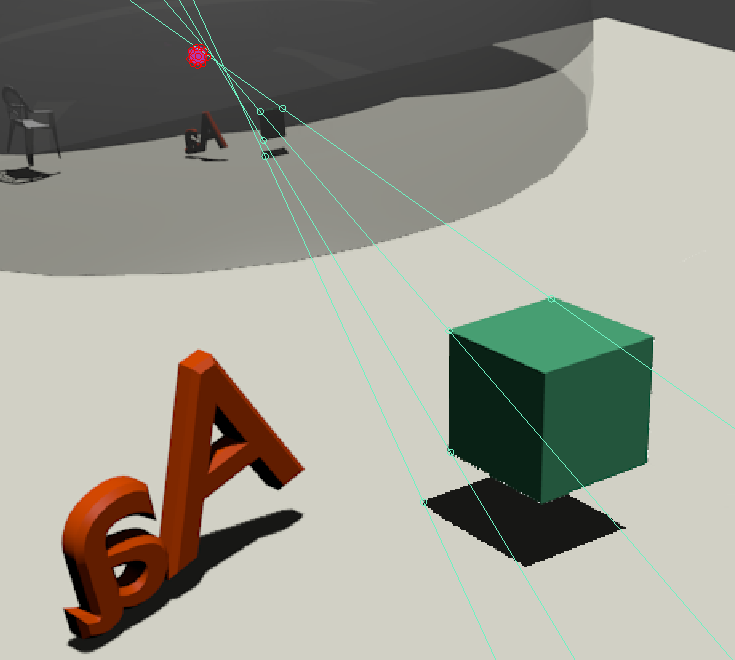
\includegraphics[width=\textwidth]{1b-lateral-reflection}
	                \caption{Movement about the sphere, with reflection also moved}
	                \label{subfig:1b-lateral-reflection}
	    \end{subfigure}
	    \\ \\
	    \begin{subfigure}[b]{0.45\textwidth}
	                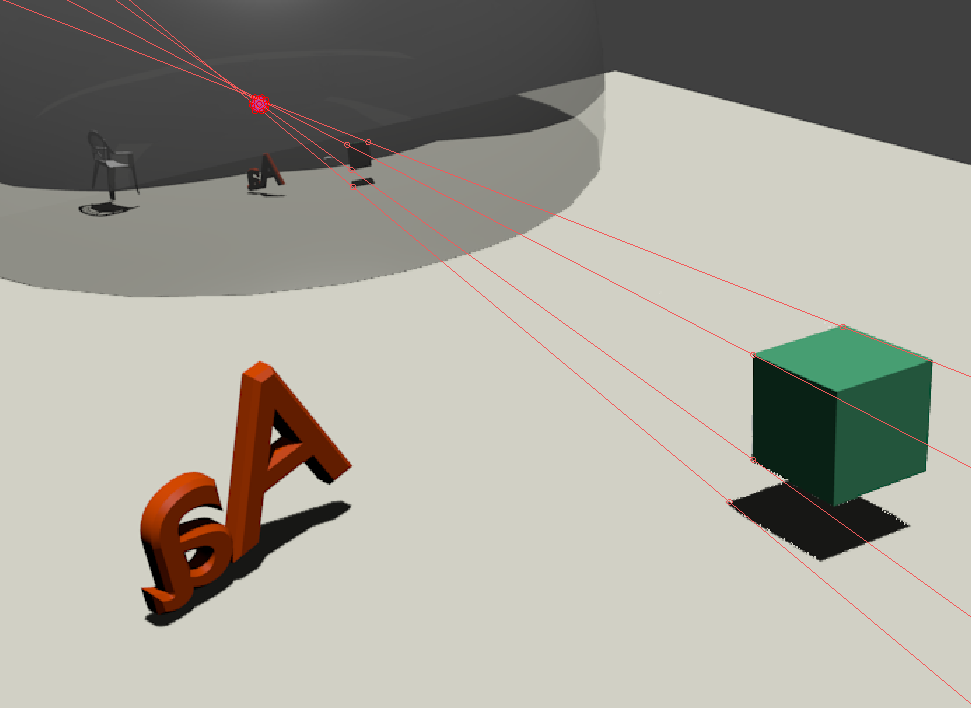
\includegraphics[width=\textwidth]{1b-away}
	                \caption{Movement away from the sphere\\}
	                \label{subfig:1b-away}
	    \end{subfigure}
	    &
	    \begin{subfigure}[b]{0.45\textwidth}
	                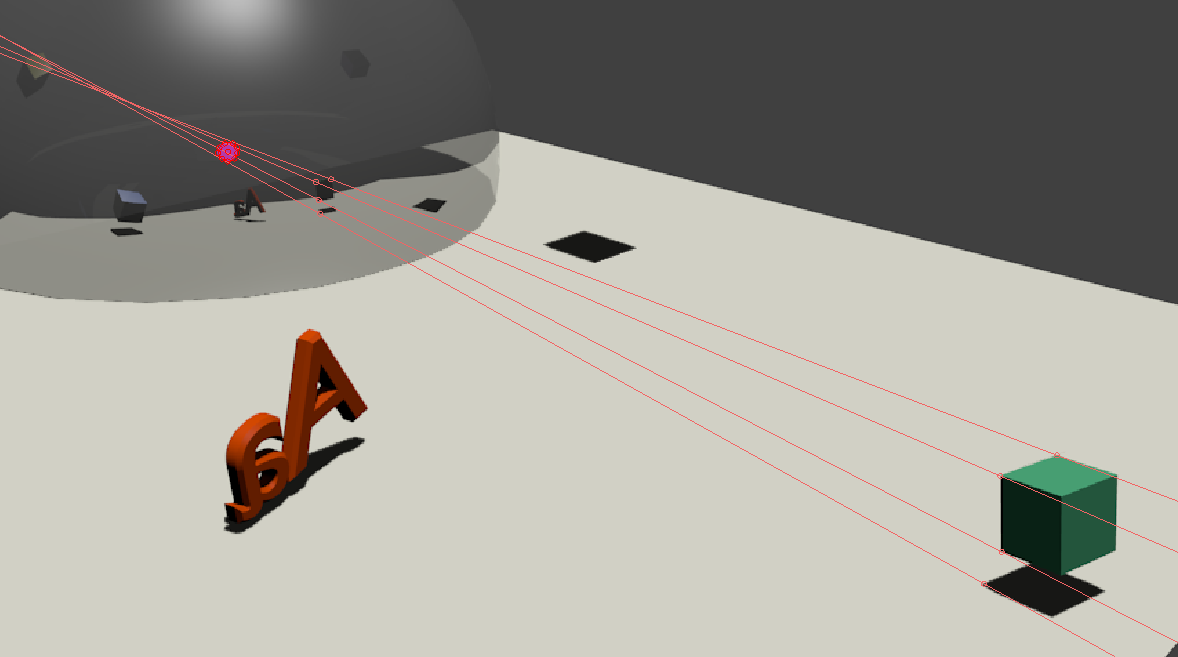
\includegraphics[width=\textwidth]{1b-away2}
	                \caption{Movement farther away from the sphere}
	                \label{subfig:1b-away2}
	    \end{subfigure}
    \end{tabular}
    
    \begin{subfigure}{0.5\textwidth}
                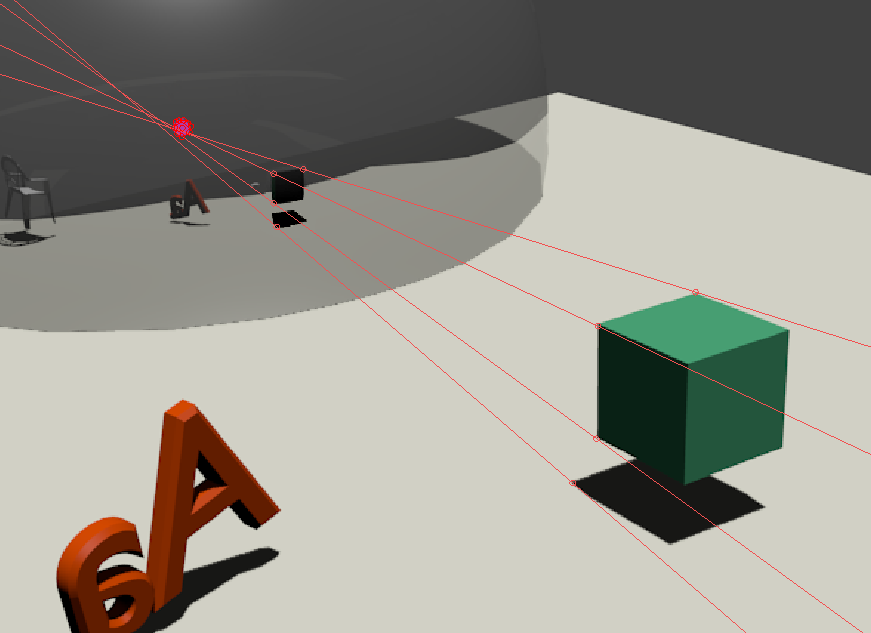
\includegraphics[width=\textwidth]{1b-composite}
                \caption{The reflection is replaced with a reflection from another image (with a smaller sphere)}
                \label{subfig:1b-composite}
    \end{subfigure}
    \caption{A comparison of different types of forgeries in which the green cube is manipulated. Original image in Figure~\ref{1b-genuine}.}
	\label{forgery-comparison}
\end{figure}

The distance-to-center test works well only in certain cases. In most cases, however, it is not sensitive enough to certain types of manipulations, which is worsened by the fact that most of the time the rays don't even intersect the sphere center for the test set.

The test is most sensitive to motion about the sphere. In Figure~\ref{subfig:1b-lateral}, the green cube is moved a distance approximately equal to its own width towards the letters. This results in a very noticeable inconsistency, as the rays lie nowhere near the sphere center. Without the rays, the image may be convincing at first glance, but on further inspection one could easily tell that the green sphere is a bit too close to the letters compared with their reflections. If the green cube's reflection is moved towards the letters' reflection as well (Figure~\ref{subfig:1b-lateral-reflection}), the rays' offset from the center is less obvious and could even be confused for the natural error that occurs in the original test images, without having the context of the original image.

Movement towards and away from the sphere is a clear weakness of the test. In Figure~\ref{subfig:1b-away}, where the green cube is moved away from the sphere by about its own width, the difference is barely noticeable aside from the rays' intersection moving to the other side of the center point. The effect is amplified if the cube is moved even farther back (Figure~\ref{subfig:1b-away2}) but if only the distances to the center are considered, this modified image is still reasonably convincing.

The most realistic scenario is one in which an object and its reflection are pasted into an image, as shifting around an object that is already there probably doesn't have many real-world applications. Figure~\ref{subfig:1b-composite} shows an image where the green cube's reflection is pasted in from a different image, in which the cube was reflected onto another sphere. Again, testing this image does not yield significant enough results to conclusively state whether or not it was manipulated, although the intersection point is not very well-defined.

One strength of both this test and almost any consistency test is that it should not produce any false positives in theory, as long as the tolerance for genuine images is calibrated correctly. It may miss some false negatives, in the case of an object moving towards or away from the sphere, but any drastic offset from the center is clearly a forgery.

\chapter{Future Work}
% counterforensics
The primary flaw in the test for rays going through the center is that there is clearly some offset in the rays, at least for the test set generated by Blender. It is possible that Blender generates the reflections inaccurately, but since the test images were generated using ray tracing (as Blender 2.37+ defaults), it is not clear how or why that would happen. In order to evaluate the validity of the test, more investigation is required into whether or not Blender truly generates images with reflections accurately, and real-life photos with spherical mirrors should be staged as well.

If applied to real-world examples, one problem that may arise is the lack of detail in the reflection, because it is likely that a spherical mirror occurring in the real world would be relatively small, and so the features of the reflection would be hard to distinguish. More research will likely be needed to determine how much detail is needed and how to enhance the reflections if necessary.

It is easy to envision that a forger could beat these techniques by performing the same tests and adjusting as needed. If they were to splice in an object and its reflection, they could align and scale them such that the projections of the incident rays go through the center of the sphere. This is limited mostly by the fact that in a real world scenario, the forger would be restricted by how the reflective surface in the source image is set up. Nonetheless, more research into counterforensics is recommended.

Finally, in order to be able to analyze most curved surfaces, methods will need to be developed to analyze reflections on other quadric surfaces, such as cylinders and cones. In these cases it would probably be necessary to develop a reliable method for estimating the normal, as these shapes are not regular as viewed from any angle as is a sphere.


\clearpage

\bibliography{Master}
\end{document}
